\section{Trigonometric Functions}


\subsection{The Unit Circle}
\begin{frame}
    \frametitle{The Unit Circle}
\begin{definition}
    The \textbf{unit circle} is the circle in the Cartesian plane with center at the origin and radius 1, defined by the equation:
    \[
    x^2 + y^2 = 1
    \]
\end{definition}                                                                                                                                    
\end{frame}


 \begin{frame}
        \frametitle{Radius corresponding to a positive angle}
        \centering
        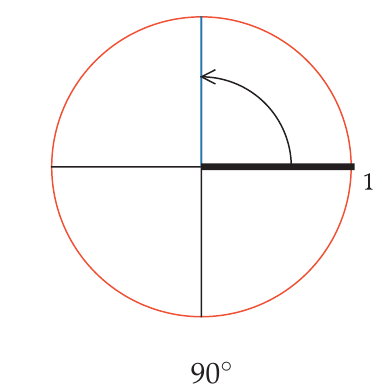
\includegraphics[scale=0.5]{/unit_circle/1.png}
    \end{frame}
    
    \begin{frame}
        \frametitle{Radius corresponding to a negative angle}
        \centering
        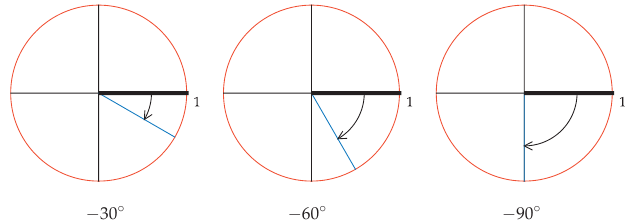
\includegraphics[scale=0.5]{/unit_circle/2.png}

    \end{frame}
    
    \begin{frame}
        \begin{block}{Positive and Negative Angles}
            \begin{itemize}
                \item Angle measurements for a radius on the unit circle are made from the
                positive horizontal axis.
                \item Positive angles correspond to moving counterclockwise from the positive
                horizontal axis.
                \item Negative angles correspond to moving clockwise from the positive hori-
                zontal axis.
            \end{itemize}
        \end{block}
    \end{frame}
    
    \begin{frame}
        \frametitle{Angles more than 360 degrees}
    \begin{block}{cyclic behaviour of angles}
        A radius of the unit circle corresponding to $\theta$ degrees also corresponds to
    $\theta + 360n$ degrees for every integer n.
    \end{block}
        \begin{figure}[h]    
            \centering
            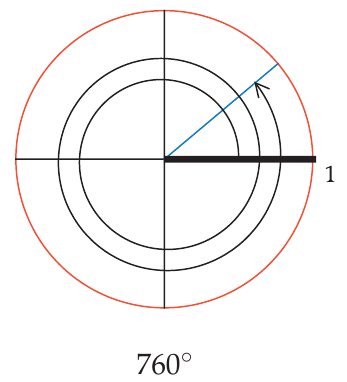
\includegraphics[scale=0.4]{/unit_circle/3.png}
        \end{figure}
        
    \end{frame}
    


    \begin{frame}
        \frametitle{Length of a Circular Arc}
        \begin{figure}
            \centering
            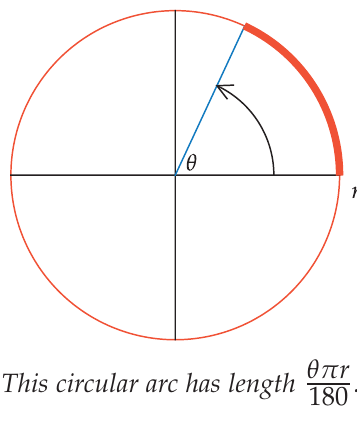
\includegraphics[scale=0.5]{/unit_circle/5.png}
        \end{figure}
        \[ 360^{\circ}   \rightarrow  2 \pi r \implies \theta^{\circ}  \rightarrow \frac{\theta}{360}.2\pi r  = \frac{\theta \pi r}{180}\] 
    \end{frame}
    
    \begin{frame}
        \frametitle{Radians}
       \begin{block}{Radians}
        Radians are a unit of measurement for angles such that $2\pi$ radians correspond
        to a rotation through an entire circle.
       \end{block}
    \end{frame}
    

    \begin{frame}
        \frametitle{Radians}
       \begin{block}{Degree to Radians}
    
        \[ 360^{\circ} = 2 \pi \text{ radians} \]
        \[ \theta ^{\circ}  = \frac{\theta \pi}{180} \text{ radians} \]
        
       \end{block}
    \end{frame}
    
    % \begin{frame}
    %     \frametitle{Arc Length}
    %     \begin{block}{length of a circular arc}
    %         If $0 < \theta \leq 2\pi$ , then a circular arc on the unit circle corresponding to $\theta$ radians
    %         has length $\theta$         
    %     \end{block}
    % \end{frame}
    
    % \begin{frame}
    %         \begin{figure}[h]    
    %             \begin{minipage}[b]{0.3\textwidth}
    %             \centering
    %             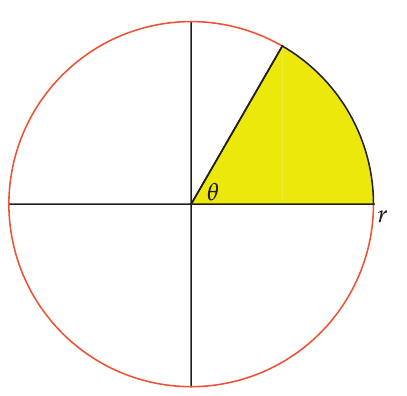
\includegraphics[scale=0.25]{7.png}
    %             \caption{Area of slice}
    %         \end{minipage}
    %     \end{figure}
    %     \begin{block}{Area of slice}
    %         A slice with angle $\theta$ radians inside a circle with radius $r$ has area $\frac{1}{2} \theta r^{2}$ .
    %     \end{block}
    % \end{frame}
    
    % \begin{frame}
    %     \frametitle{Cosine and Sine}
    %     \begin{figure}[h]    
    %         \begin{minipage}[b]{0.8\textwidth}
    %         \centering
    %         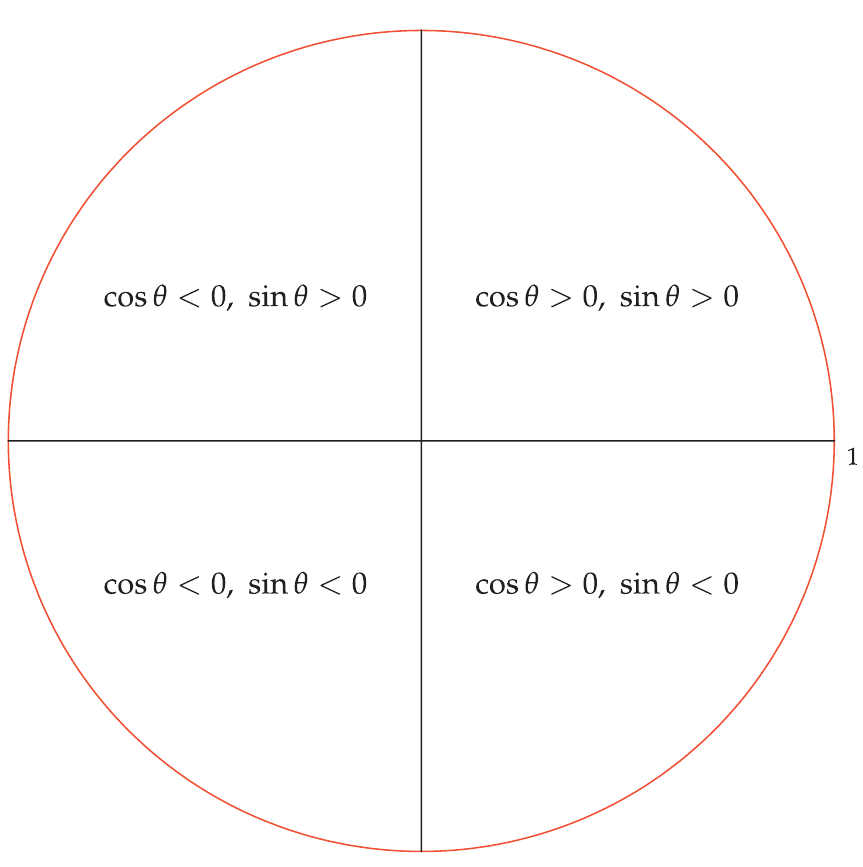
\includegraphics[scale=0.22]{8.png}
    %         \caption{sin and cos}
    %     \end{minipage}
    % \end{figure}
    % \end{frame}
